%!TEX root = /Users/Nikolaj/Developer/GPU-Project/Report/Report.tex
The following two sections describes the two CUDA implementations made during this project. The first implementation attempt, MiddlePar, was the first iteration on how we could parallelize the mathematical model described earlier. The second implementation attempt, OuterPar, is an improved version of the first attempt that further parallelize. Both CUDA implementations derive directly from the C implementation described earlier.

\subsection{First Attempt: MiddlePar}
In order to parallelize the C implementation and make use of the parallelism of the GPU, we had to analyze the each model of the implementation. Our approach was to locate the most obvious part that could be parallelized, and developed a CUDA version of that. Since the solution could not be parallelized entirely, we acknowledged that some calculations would be done on the GPU, the parts that could be parallelized, and the rest would be run on the CPU. The most obvious possibility for a CUDA solution is found within the middle model. Compared to both the outer and the inner model, the steps within the middle model were not dependent on the previous steps. \texttt{Middle(...)} is calculated by adding the result of $k1$, $k2$, $k3$, $k4$ and then add it with the y value of the previous step. This means that for each step we can calculate the sum of all the $k$ values before we add it all together. This is a good start since the calculation of either $k$, is essentially a call to the inner model. This solution would keep the amount of inner model calls per thread to be only 4. The MiddlePar CUDA implementation is explained in the following section.

\subsubsection{Implementation} \hfill\\
The implementation of this CUDA solution is apparent in the method \texttt{OuterDi-\\ff(..)}, which is the method that needs a result from the middle model. \texttt{OuterDiff(..)} prepares two variables that is to be copied to the GPU. The first is the current $x$-value from outer, that is needed to calculate \texttt{Middle(...)}, and an array called \texttt{kSum}. This array will be used to store the sum of $k1$, $k2$, $k3$ and $k4$, calculated by each thread. Having these results, calculating each step in \texttt{Middle(...)} can be done much faster, since it is just a matter of adding two double values together for each step. \\ \\

Based on the step size it is possible to calculate exactly how many steps \texttt{Middle} needs to take. Prior to starting the kernel, we need to make sure that there are enough threads available when parallelizing \texttt{Middle}, such that there are at least one thread for each step. The amount of threads per block would be set prior to program execution, and before starting the kernel the amount of blocks needed to ensure enough threads would be automatically calculated.\\

In the following we will explain the kernel implementation; see figure \ref{fig:middlepar} for the changes made to \texttt{Middle(...)}. \\
\begin{figure}[H]
\begin{lstlisting}[language=c]
__global__ void Middle(double *t, double *kSum){
	int tid = threadIdx.x + blockIdx.x*blockDim.x;
	//constData[4] refers to the h2 constant
	double stepsize = -1 / constData[4]; 
	//constData[6] refers to the level2fullsteps constant
	const int fullsteps = constData[6]; 
	if(tid<fullsteps){
		double gt = *t; //de-reference input
		//constData[0] refers to the x constant
		double tau = constData[0] + gt; 
		double kk = k(tau);
		double eta = (120+(tid*stepsize));
		double k1 = stepsize * MiddleDiff(tau, eta, Inner(eta, gt, kk).y);
		double k2 = stepsize * MiddleDiff(tau, eta + stepsize/2, Inner(eta + stepsize/2, gt, kk).y);		
		double k4 = stepsize * MiddleDiff(tau, eta + stepsize, Inner(eta + stepsize, gt, kk).y);
		kSum[tid] = k1/6+k2/3+k2/3+k4/6;
	}
}
\end{lstlisting}
\caption{The kernel code for \texttt{Middle} in MiddlePar}
\label{fig:middlepar}
\end{figure}

Once the kernel has been started, each thread define their global thread id by calculating $threadIdx.x + blockIdx.x \times blockDim.x$. This ensures that each thread within the kernel has a unique id, which we will need later on.\\

We then ensure that only threads, that have an id within the range of middle steps, continue on from line 7 in figure \ref{fig:middlepar}. We know that this will cause branch diversion in the last block if the total amount of threads is not equal to the amount of steps, however this is a necessary precaution as we will see soon.\\

The next couple of lines is used to calculate local variables, that is used to call both \texttt{Inner(…)} and \texttt{MiddleDiff(…)}. $k1$, $k2$ and $k4$ is then calculated by calling \texttt{MiddleDiff(…)} and \texttt{Inner(…)}. In line 16 the weighted average of each $k$ is calculated and stored in the \texttt{kSum} array. This is where it is important that the thread id does not exceed the amount of steps. The size of \texttt{kSum} is exactly the total amount of steps, so if a thread id is larger than this, we would run into problems. A solution could be to always make sure that the number of threads you have is equal to the amount of steps to be taken, however since both threads per block, as well as middle steps, varies it is not feasible, and cannot always be ensured. Once the sum of the $k$ values have been stored in \texttt{kSum} for all threads, the kernel terminates.

\subsubsection{Memory considerations} \hfill \\
This CUDA implementation accesses certain constant variables quite a lot when calculating \texttt{Inner(…)}. Since we were ever only going to read these constants, it would be a good idea to place this information in constant memory. Constant memory is considerably faster than global memory(INSERT REF), with the limitation.\\

It was also considered to keep \texttt{kSum} in shared memory. Shared memory, like constant memory, is likewise considerably faster than global memory, however it is possible for more than one block to be part of the kernel execution. Shared memory allows thread within the same block to share data, but not between blocks, so shared memory was discarded for this solution, and \texttt{kSum} was kept in global memory.

\subsubsection{Implementation shortcomings} \hfill \\
\label{label:shortages}
The solution described above has a few drawbacks. First of all, each time a call to \texttt{Middle(...)} is made, a new GPU context would be set up, variables would be copied to the GPU, and a new kernel would be started. Doing this for a low $x$-value, and a high stepsize, would result create a large amount of kernels. Second, this solution needs more than one block to parallelize \texttt{Middle(..)} if the amount of threads per block were low. Even though it would speed up the call to \texttt{Middle(...)}, it does not speed it up the amount of total calls made to \texttt{Middle(...)}. Third, we are not using a lot of threads or blocks to actually make the calculations, compared to how many threads and blocks are available on modern GPUs. Fourth, it would be much more efficient to use shared memory for storing the \texttt{kSum} array, instead of keeping it in global memory.\\

We could of course address some of these issues, but since we are going to improve this implementation in the next section, it was decided not to further alter this implementation. \\

\subsection{Second Attempt: OuterPar}
To address the shortcomings the GPU parallelization of \texttt{Middle(...)}, we would have have to make some major changes to the existing GPU and CPU code. First we need to make sure that \texttt{Middle(...)} is ever only being calculated using the threads from within a single block. We also needed to change \texttt{kSum} to be a shared variable array instead of an input array. \\

Furthermore we had to parallelize the total calls to \texttt{Middle(...)}. Investigation showed that the differential equation of the outer integral used only the current $x$-value from the outer steps to calculate \texttt{Middle(...)}. This effectively meant that we could calculate all $x$-values in advance (we knew the start $x$-value, the end $x$-value as well as the size of each step), and further calculate all calls to \texttt{Middle(...)} in advance using these values. These could all be calculated at once on the GPU using only one kernel. Together with the changes to \texttt{Middle(...)} this would allow us to run several blocks to calculate different \texttt{Middle(...)} calls at the same time and make better use of the GPU resources. The CUDA implementation is described in the following section.

\subsubsection{Implementation} \hfill \\
The first changes were made in \texttt{Middle(…)}. The changes were made to address two of the issues described in \ref{label:shortages}, regarding the use of multiple blocks within a single call \texttt{Middle(…)}, as well as the lack of a shared variable to store \texttt{kSum}. Figure \ref{fig:outerpar} shows the updated code. The first two changes is easily  visible. Since all threads that will calculate each step in \texttt{Middle(…)} is now always within the same block, we can define a shared variable (for much faster data storing) \texttt{kSum}, and we can define the thread id to be simply the id within the block (INSERT CORRECT LINE AND FIGURE).\\

\begin{figure}[ht]
\begin{lstlisting}[language=c]
__global__ void Middle(double *outerx, double *temp){
	extern __shared__ double kSum[];
	int tid = threadIdx.x;
	double stepsize = -1 / constData[4];
	const int fullsteps = constData[6];
	double gt = outerx[blockIdx.x];
	while(tid<fullsteps){
		double tau = constData[0] + gt;
		double kk = k(tau);
		double eta = (120+(tid*stepsize));
		double k1 = stepsize * MiddleDiff(tau, eta, Inner(eta, gt, kk).y);
		double k2 = stepsize * MiddleDiff(tau, eta + stepsize/2, Inner(eta + stepsize/2, gt, kk).y);		
		double k4 = stepsize * MiddleDiff(tau, eta + stepsize, Inner(eta + stepsize, gt, kk).y);
		kSum[tid] = k1/6+k2/3+k2/3+k4/6;
		tid = tid + blockDim.x;
	}
	tid = threadIdx.x;
	__syncthreads();
	if(tid == 0){
		double y = 0.0;
		int i;
		for(i = fullsteps-1; i>=0; i--){
			y = y+kSum[i];
		}
		temp[blockIdx.x] = y;
	}
}
\end{lstlisting}
\caption{The kernel code for \texttt{Middle} in OuterPar}
\label{fig:outerpar}
\end{figure}

The next change is that we can get the $x$-value from outer, from a pre-calculated array, \texttt{outerx}, passed to the kernel at execution time. The $x$-value needed for a specific block can then be accessed by indexing on the unique block id(INSERT CORRECT LINE AND FIGURE).\\

We further changed the if statement to a while loop and added a counter. Since the number of threads per block can be less than the number of steps to be taken, we want to ensure that threads iterate over multiple steps instead of just one, such that \texttt{kSum} will be correctly filled. It also ensures that if a block contains more threads than there are steps to be taken, they do not enter the while loop. Apart from the counter, everything within the while loop is the same as it was in figure \ref{fig:middlepar}.\\

The next part of the code was done in \texttt{OuterDiff(…)} for the MiddlePar solution. This was because, when working with multiple blocks, one could never guarantee that all blocks had reached the same part of the code before moving on. The only situation where you know for certain that all blocks have finished execution is when the kernel terminates. For the MiddlePar solution we copied \texttt{kSum} back to the CPU and made it compute the sum there. However, now that we are only working within a single block we can make use of the \texttt{\_\_syncthreads()} statement (line 18 in figure \ref{fig:outerpar}). This statement ensures that all threads (within the same block) have reached this line of code before continuing. We also reset the thread id in case we had to loop in line 17 in figure \ref{fig:outerpar}. \\

Once we have calculated \texttt{kSum} for each thread we need to add it together to a single value. There are basically two ways to do this; using a single thread to iterate over all the values in \texttt{kSum} and add them together, or using reduction(insert CUDA by example reference). Reduction is a method where you make use of the threads already available, and have them add two values together, until you only have one value left. See figure \ref{fig:reduction} for a visualization of this concept. This allow the sum of \texttt{kSum} to be computed in $log2(threadsperblock)$ iterations.\\

\begin{figure}[ht!]
  \centering
    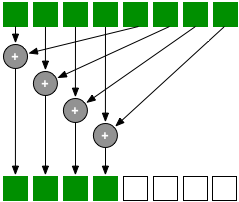
\includegraphics[scale=0.5]{Reduction}
  \caption{Reduction (INDSÆT REF)}
  \label{fig:reduction}
\end{figure}

Reduction seems like the most obvious choice, however there is a downside. For reduction to work you need an array, and a number of threads that are a power of 2 (insert CUDA by example reference). We can make sure that the number of threads per block is always a power of 2, however we can never guarantee that the same goes for the size of \texttt{kSum}. The size of \texttt{kSum} is 119 times the stepsize, and for good reasons this can never be guaranteed to be the power of 2. A solution to this would be to always make sure that the size of \texttt{kSum} is the power of 2, and then just fill the unused elements with zeros. However this overhead meant that we might as well just loop through \texttt{kSum} and sum everything together with a single thread. We therefore decided not to use reduction in this case.\\

Once the sum has been calculated it is stored in the input array temp using the block id for indexing. Once all blocks have executed, the kernel terminates and temp is copied back to the CPU. When \texttt{OuterRK(…)} is called from this point on, instead of calling \texttt{Middle(…)} whenever it solves the integral, it just indexes into temp.

\subsubsection{Memory considerations} \hfill \\
Just like the MiddlePar implementation this CUDA solution access certain constant variables quite a lot when calculating \texttt{Inner(…)}, and for this solution it further accesses the constants for \texttt{Middle(…)} a lot. Since we were ever only going to read these constants, we kept them in constant memory.\\

However compared to the MiddlePar solution \texttt{kSum} was now kept in shared memory instead of global memory, which were made possible due to the changes we made to \texttt{Middle(…)}. Writing to this array should now be faster than the previous solution, as we can access the array much faster.

\subsection{Profiling and comparison}
\subsubsection{Nvidia visual profiler result} \hfill \\

The following results were gathered using Nvidias Visual Profiler for analyzing both the MiddlePar and OuterPar CUDA implementation. First we will present the results and then we will discuss them in the next section.
\begin{savenotes}
\begin{table}  
\begin{center}
\begin{tabular}[t]{|c|c|c|}
	\hline
\textbf{Attributes} & \textbf{MiddlePar} & \textbf{OuterPar} \\\hline
Grid size  & 2,1,1 & 1700,1,1\\\hline
Block size & 128,1,1&128,1,1\\\hline
Registers/thread & 62&63\\\hline
Shared Memory/Block &0 bytes& 1904 bytes \footnote{The visual profiler wrote that OuterPar used 1859 bytes of shared memory. This is however wrong. The command line profiler showed the correct result. The result can be calculated as 119*h2*8, which in this case is 119*2*8 = 1904 bytes.}\\\hline
Global Load Efficiency \footnote{We assume that at maximum we can achieve 100\% efficiency and not above.}&86,2\%&764.5\%\\\hline
Global Store Efficiency&99,2\%&25\%\\\hline
Branch Divergence Overhead&21.9\%& 21.8\%\\\hline
Occupancy \footnote{According to the profiler the theoretical occupancy is 33.3\%}&6.5\%&33.1\%\\\hline
\end{tabular}
\end{center}
\caption{Nvidia Profiler Results. Input: g=10, r=65, x=35, h1=10, h2=2, h3=10, threadsPerBlock=128.}
\label{table:profiler}
\end{table}
\end{savenotes}

\subsubsection{Comparison and discussion} \hfill \\
It is evident from the results in table \ref{table:profiler} that there are some major differences in the two implementations. Namely grid size, occupancy and global load store.
\\ \\
The difference in grid size make sense, when considering the implementation differences. MiddlePar seeks to parallelize a single call to Middle, whereas OuterPar tries to compute all middle calls at once. Therefore the amount of blocks in MiddlePar depends on the number of threads per block, and the amount of steps to be taken in middle. In worst case, this would require 38 blocks to cover a middle stepsize of 10 and 32 threads per block\footnote{If stepsize is 10 we need to take 119*10 steps, and with 32 threads per block we would need ceil(119*10/32) blocks to cover all steps}. This stands in large contrast to the amount of blocks used by OuterPar. The difference is thus that in MiddlePar we will create a huge number of kernels when executing the program, where the kernel is run once with OuterPar.
\\ \\
From this, the difference in occupancy is also evident. Running a very small number of blocks with a small number of threads is only going to use a small part of the GPU. Furthermore whenever warps fetch data from global memory during the MiddlePar execution, storing to global memory waiting for a FLOP to finish, there are almost no warps to take its place while it waits. This means that the SM's that have blocks assigned will be idle (further lowering occupancy). During OuterPar execution there are enough blocks to assign the full number of blocks per SM's on the GPU. Furthermore whenever a block finishes execution, there are several blocks waiting to be assigned to a SM leaving very little time to stand idle. The time the SM's will start to idle will begin towards the end when there are no more blocks waiting in the pipeline. All together this means that the GPU will be fully occupied during most of the kernel execution.
\\ \\
Global load store efficiency is different for the two programs for a very simple reason. Where most of the threads in MiddlePar writes to global memory, only a single thread per block writes to global memory in OuterPar. Whenver a request to store to global memory is initiated the the SM tries to write the minimum amount of bytes possible which is 32 bytes. Since we are only storing a single double value (8 bytes), only 25\% of the store request is actually used.